\section{Methods}
\label{ch:TugOfWarMethods}

To justify the choice of relevant forces in mass-spring model, we used available literature values to estimate the generated forces in application to capsid protein M1 (Appendix \ref{appendix:nanomolecular}). As a result, in this model we focus on capsid stiffness and forces generated by tug-of-war between molecular motors.

The mass-spring mathematical model for capsid breakage represents a rectangular fragment of the capsid at the stage when it is exposed via the fusion pore and is interacting with host molecular motors, which pull it apart (Figure \ref{figure:fluMassSpring}A).

Capsid M1 proteins (the masses) are arranged in a regular mesh approximately of the size of the fusion pore (see Appendix Table \ref{table:MassSpringParameters} for all parameter values). Edge nodes of the mesh are bound to the lipid bilayer of the viral envelope/endosome and inner nodes are exposed to the cytoplasm. Here, we used a 6x6 mesh with 4x4 inner capsid proteins. Each inner mass is computed as the sum of protein masses bound to a particular node. For example, a free capsid node would simply correspond to the M1 protein mass, while a node attached to a myosin motor would have a total mass equal to the sum of masses of M1 protein, HDAC6, Ub, and myosin. Each edge node mass is the average mass of the endosome divided by the number of edge nodes.

The masses are connected to each other with elastic bonds, which we represent as a Morse potential that can explicitly include effects of bond breaking. Specifically, the Morse potential is

\begin{equation}
V_{Morse} (r) = D_e \big(1 - \exp(-a(r - r_e)^2)\big)
\end{equation}

where  $a = \sqrt{\frac{k^2_e}{D_e}}$, which has two parameters: stiffness $k_e$ and dissociation energy $D_e$. In this model we use two sets of Morse parameters for inner and outer nodes.

Each of the inner nodes of the capsid is acted on by the elastic forces of the 4 springs connecting it to other nodes. We calculate the change in spring length between two nodes as

\begin{equation}
\delta l = \sqrt{(\delta x)^2 + (\delta y)^2} - l_{equilibrium}
\end{equation}

where $\delta x = x_{neighbor} - x_{current}$ and $\delta y = y_{neighbor} - y_{current}$ are the differences between the x and y coordinates of the neighbor node and the current node, and $l_{equilibrium}$ is the equilibrium spring length. The change in spring length $\delta l$ determines the force acting on the node, created by each particular spring. We compute the force as

\begin{equation}
f_{Morse spring} = -2 a^{type} D^{type} \exp(-a^{type} \delta l) \big(1 - \exp(-a^{type} \delta l)\big)
\end{equation}
 
where $a^{type}$ and $D^{type}$ are the parameters of the Morse spring, depending on the spring’s type (inner nodes corresponding to capsid parameters and edge nodes to capsid with lipid bilayer cover).

We then compute the projections on the x and the y axis of the acceleration created by each of the spring forces as follows:

\begin{equation}
a^{spring}_z = \frac{f_{Morse spring}}{m_{node}} \Big(\frac{-\delta z}{(\delta x)^2 + (\delta y)^2}\Big)
\end{equation}

where $m_{node}$ is the node’s mass and $z$ stands for either $x$ or $y$.

Finally, the ODE system for one node looks as follows

\begin{equation}
\frac{d}{dt}
\begin{pmatrix}
c_x\\
c_y\\
v_x\\
v_y
\end{pmatrix}
=
\begin{pmatrix}
v_x\\
v_y\\
a^{top}_x + a^{right}_x + a^{bottom}_x + a^{left}_x + \frac{f^{motor}_x}{m_{node}}\\
a^{top}_y + a^{right}_y + a^{bottom}_y + a^{left}_y + \frac{f^{motor}_y}{m_{node}}
\end{pmatrix}
\end{equation}

where $c_x$, $c_y$ denote x and y coordinates of a node, respectively, and $v_x$, $v_y$ denote x and y velocities of a node, respectively. 

We model the cytoskeleton near the fusion pore by a single, randomly directed microtubule, and by a denser network of actin filaments with a nucleation point on one of the edge nodes. Molecular motors are directly or indirectly (which we do not distinguish in this model) connected to the exposed capsid M1 proteins and to the cytoskeleton, allowing them to exert forces on the capsid. Specifically, dynein motors can walk in a single direction along the microtubule, while myosin motors can walk along actin filaments in random directions away from the nucleation point. Dyneins can connect to any of the inner nodes, but they can only exert forces on the capsid if they fall within the microtubular area of effect, determined by its width (Figure \ref{figure:fluMassSpring}A).
We compute the resulting forces through a tug-of-war model with experimentally determined motor characteristics \cite{gennerich2007force, muller2008tug, norstrom2010unconventional}, which we modified to represent dyneins, kinesins, and positive- and negative-direction myosins. Importantly, the model considers that the force exerted by each individual motor depends on all the other motors bound to the same cargo, and assumes that forces exerted by the motors are proportional to their respective stall forces. The detailed derivation of two dimensional tug-of-war equations is described in Appendix \ref{appendix:2DTugOfWar}.
 
To avoid division by zero, in simulations we assume that there are always one dynein and one kinesin bound to the endosome outside of the fusion pore because the endosome had to be transported inside the cell to initiate fusion pore formation. Due to the architecture of the Tug-of-War model and since all the microtubular motors can only generate forces along the microtubule, adding more endosomal motors would simply offset the optimal amount of dynein motors required for efficient breakage. All other motors are bound to the capsid from the very start of the simulation.
 
During simulations of the mass-spring model, each motor configuration has a fixed number of each type of motor, but the placement and the directions of cytoskeletal filaments are randomized. The model is simulated for one microsecond of system time at least 100 times for each motor configuration using the MATLAB ODE solver ode15s (Mathworks, Natick / MA).

After a simulation, we examine the distance between all neighboring nodes in both $x$ and $y$ directions. If during the simulation the combined motor forces were sufficient to make any of the distances exceed the RNP complex diameter (a mock-up example for the one-dimensional case of break/no break scenarios showed in Figure \ref{figure:PersistentBreaks}) for at least half the simulated system time (to avoid counting transient breaks), we classified the capsid as broken. Usually, however, if capsid breakage occurs, the initial break happens early in the simulation and persists through 80-90\% of the simulation time (Figure \ref{figure:BreakDuration}).

\begin{figure}
\begin{center}
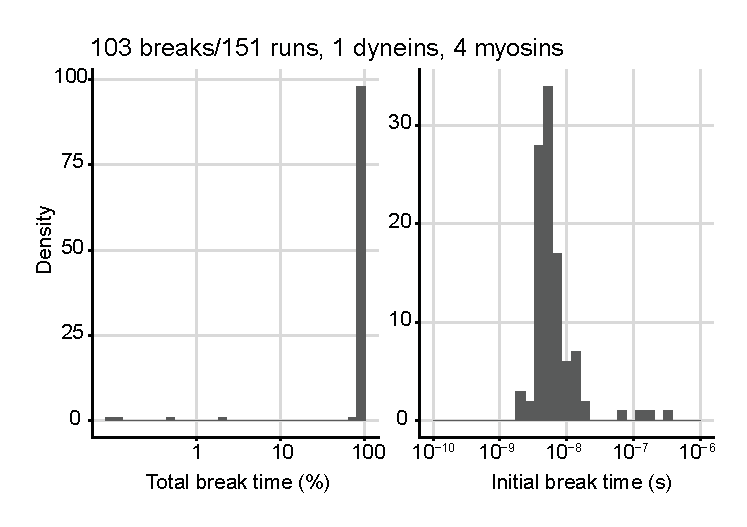
\includegraphics[width=0.95\textwidth, trim={0cm 0cm 0cm 0cm}, clip]{D_chapters/1_TugOfWar/SUPPLEMENTARYFIGURE1B.pdf}
\caption[Most simulations that achieve a break have it occur early and persist for most of the simulation]%
{Most simulations that achieve a break have it occur early and persist for most of the simulation. \par
The total break time (fraction of time points in which the system is broken) and initial break times for simulations where breakage occurred for a 4x4 grid with one dynein and four myosin motors. Most simulations that achieve a break have the initial break early on (~10-8 s, for a total 10-6 s simulation time).}
\label{figure:BreakDuration}
\end{center}
\end{figure}

To analyze the robustness of the simulation results to changes in capsid parameters, we fixed a combination of motors (5 myosins and 1 dynein) that produced approximately 50\% breakage, and varied the capsid bond parameters stiffness $k_e$ and dissociation energy $D_e$. The values used in our simulations were $k_e \in$ [0.001, \textbf{0.002}, 0.003, 0.004, 0.005] N/m and $D_e \in$ [10, 12, \textbf{14}, 16, 18, 20] kJ, where boldface indicates the default values (Figure \ref{figure:StiffnessEnergy}).

To simplify computation of the capsid breakage probability, we interpolated it as a function of the total amount of molecular motors and the number of dynein motors using the R package akima on the basis of the values obtained from simulation of the mass-spring model (Figure \ref{figure:MassSpringInterpolation}).

\begin{figure}
\begin{center}
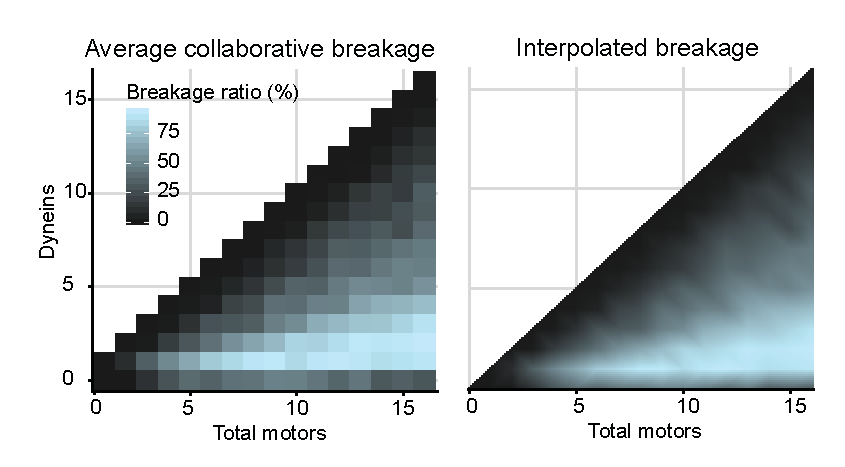
\includegraphics[width=0.95\textwidth, trim={0cm 0cm 0cm 0cm}, clip]{D_chapters/1_TugOfWar/SUPPLEMENTARYFIGURE1D.pdf}
\caption[Collaborative breakage by molecular motors and the interpolated capsid breakage probability]%
{Collaborative breakage by myosin and dynein motors (left) and the interpolated capsid breakage probability (right) that is used in Chapter \ref{ch:ReactionModels} to estimate capsid breakage in the reaction model.}
\label{figure:MassSpringInterpolation}
\end{center}
\end{figure}